\subsection{Brief Design Specification}
\subsubsection{Overall summary description of the module}
Part 1 of the lab requires us to blink LEDs, and control their patterns by programs or a button. A communication between Arduino board and computer is also covered. To meet this requirement, we need to set the pins and their modes correctly, then program the processor to receive input, control the flow, and send output. Besides, we need to set up the connection between processor and computer. Test text will be sent to ensure it works correctly, and then the processor should do a calculation and send out the result.\\
In part 2, we will need a module that can work with the LCD and two modules that can communicate, which reflects on the control of the LED of one microprocessor by another. To meet the requirement of being able to work with the LCD, we need the correct control of the content, situation, and moving of the characters printed on the LCD by the module. To meet the requirement of being able to communicate, we need to send data correctly from the master microprocessor to the slaver microprocessor.
\subsubsection{Specification of the public interface to the module}

\paragraph{Input, Output and Side Effects}
\subparagraph{lab 1 \& 2}
There is no input in this program. The output is the blinking of LED on the board, which follows a pattern we set before. 
\subparagraph{lab 3 \& 4}
This part is much like the one above, with the output device here being an LED brick instead of onboard LED. It blinks in two ways under the control of the program.
\subparagraph{lab 5}
We have connected a button brick to the board so whether it is pushed or not becomes the input signal. The output is the blinking of the LED brick, which is controlled by the brick.
\subparagraph{lab 6 \& 7}
In this part we are trying to use the processor output, so output is the information through serial. Program 6 prints some preset words on the serial monitor and Program 7 prints our own stuff. There is no input.
\subparagraph{lab 8} 
No input is required, the output is the LCD connected to the microprocessor printing two names on the first row of the display and one on the second.
\subparagraph{lab 9}
The input is controlled by two peripheral buttons, which can generate high signal by being pressed, and the output is the cursor on the LCD display moving left if one of the button is pressed and to the right if the other is pressed. If the cursor meets the end of the two rows of the LCD display, it will show up at the first column of the second row and can be controlled again.
\subparagraph{lab 10}
No input is required, and the output is detected on the Serial Monitor on the PC. If the Serial Monitors of the two microprocessors are opened separately, the slaver's monitor should display the same number series as the master's does. 
\subparagraph{lab 11}
The input is controlled by a peripheral button brick connected to the master microprocessor, and the output is the peripheral LED connected to the slaver microprocessor being turned on when the button is pressed, and turned off when the button is released.
\paragraph{Pseudo English description of algorithms, functions, or procedures}
\subparagraph{lab 1 \& 3}
set LED as output;
loop while true\{
	set the voltage high;
	wait for 2 seconds;
	set the voltage low;
	wait for 1 second;
\}
\subparagraph{lab 2 \& 4}
set LED as output;
loop while true\{
	two-second blink;
	one-second blink;
	two-second blink;
	two-second blink;
\}
\subparagraph{lab 5}
set LED as output;
set button as input;
loop while true\{
	if (button pushed)\{
		LED on;
	\}
	else\{
		LED off;
	\}
\}
\subparagraph{lab 6}
set an integer;
start serial port;
loop while true\{
	serial print "hello world";
	serial printline i;
	wait 1 second;
	serial printline "how ya doin";
	wait 1 second;
\}
\subparagraph{lab 7}
start serial port;
serial printline some own stuff;
\subparagraph{lab 8}
print the name of first two members;
move the cursor to the first column of the second row;
print the name of the third member;
\subparagraph{lab 9}
row = 0;col = 0;
connect the input pins to variables respectively;
if the variable related to the left button is high, and if cursor is at the beginning of the second row, move the cursor to the end of the first row, if it is at the beginning of the first row, do nothing, else col -=1 ;
if the variable related to the right button is high, and if cursor is at the end of the second row, move the cursor to the beginning of the second row, if it is at the end of the first row, move it to the beginning of the second row, else col +=1 ;
keep doing the checking process with a delay of 300 in each round;
\subparagraph{lab 10}
Although the code for this lab is provided on the course website, we will still present the pseudo code.
x = 0;
set the correct output port;
send the value of x ; x��+= 1;
keep the sending and adding process, with a delay in each round;
\subparagraph{lab 11}
lightOn = 0;
connect the variable lightOn to the control pin of the LED light in the slaver module;slaver module keeps receiving the signal from the master microprocessor and saves its correspondent value into lightOn.
if the button is pressed, the master sends a byte string representing that the light is on to the slaver, if not, it sends a byte string representing that the light is off to the slaver.
\subsection{Hardware Implementation}
See figure 1 for details.
\begin{figure}
	\centering
	\label{fig:1}
	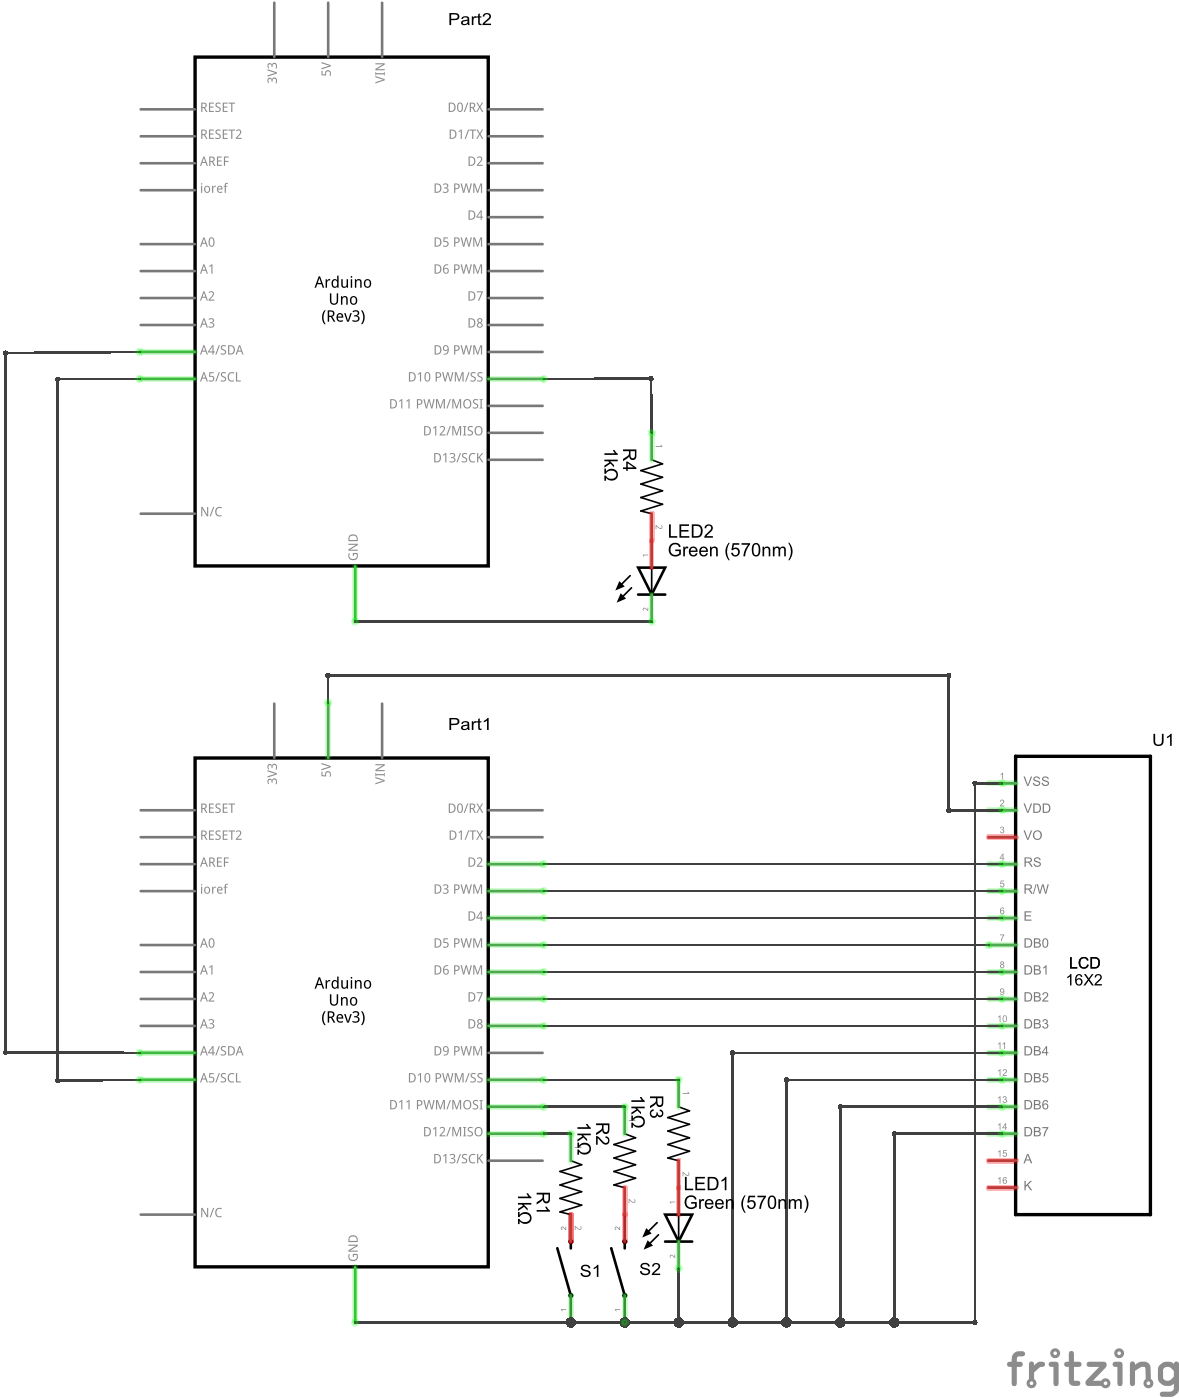
\includegraphics[width = \linewidth]{images/harware_schem.png}
	\caption{Schematic of hardware implementation(developed using Fritzing)}
\end{figure}
%\subsection{Software Implementation}